\appendix

\chapter{Appendix} \label{chapter:appendix}

\section{Source Code and Data}
The source code of the thesis is available on GitHub split in two repositories. Both repositories have Readme files that explain how to use the code and data. 
\begin{itemize}
    \item \textbf{Prototype Repository:} Contains the implementation of the APR Core and the CI configuration. It is available at: \url{https://github.com/justingebert/bugfix-ci}
    \item \textbf{Evaluation Repository:} Contains the evaluation scripts and results of the APR system, including the QuixBugs benchmark setup. It is available at: \url{https://github.com/justingebert/quixbugs-apr}
\end{itemize}


\section{LLM Versions}
The following Table lists the exact LLM versions that where used during development and evaluation. 
\begin{longtable}{p{5cm} | p{6cm}}
    \caption{LLM models and their versions used in the system} \label{table:llm_versions} \\
    \hline
    \textbf{Model Name} & \textbf{Version} \\
    \hline
    \endfirsthead
    \hline
    \endfoot
    gemini-2.0-flash-lite    & gemini-2.0-flash-lite \\
    gemini-2.0-flash         & gemini-2.0-flash \\
    gemini-2.5-flash-lite & gemini-2.5-flash-lite-preview-06-17 \\
    gemini-2.5-flash         &  gemini-2.5-flash\\
    gemini-2.5-pro           & gemini-2.5-pro \\
    gpt-4.1-nano             & gpt-4.1-nano-2025-04-14 \\
    gpt-4.1-mini             & gpt-4.1-mini-2025-04-14 \\
    gpt-4.1                  & gpt-4.1-2025-04-14 \\
    o4-mini                  & o4-mini-2025-04-16 \\
    claude-3-5-haiku         & claude-3-5-haiku-20241022 \\
    claude-3-7-sonnet        & claude-3-7-sonnet-20250219 \\
    claude-sonnet-4-0        & claude-sonnet-4-20250514 \\
    \hline
\end{longtable}

\newpage

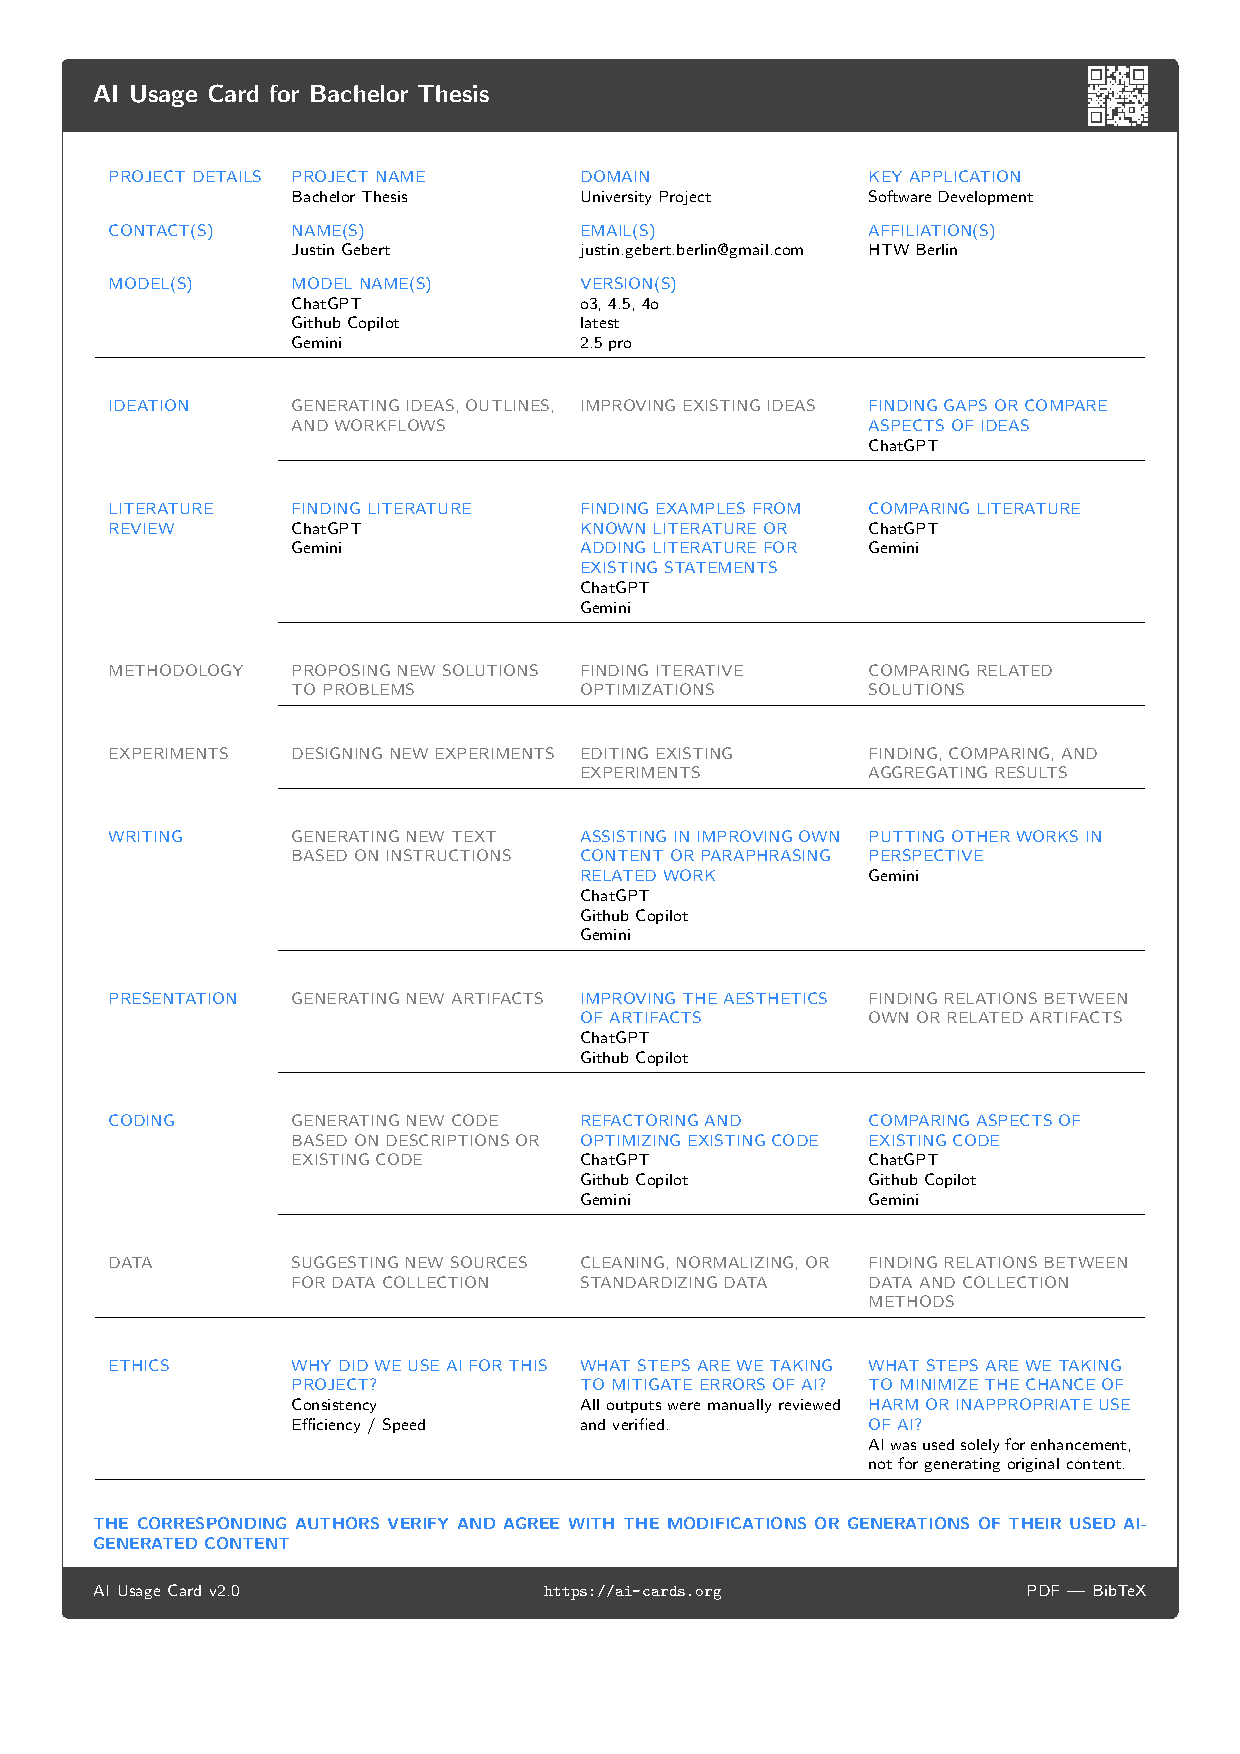
\includepdf[pages={1}]{pages/Ai-usage-card.pdf}

\thispagestyle{empty}
%\vspace*{18cm}
\noindent


\section*{Eidesstattliche Versicherung}
Hiermit versichere ich an Eides statt durch meine Unterschrift, dass ich die vorstehende Arbeit selbstst\"andig und ohne fremde Hilfe angefertigt und alle Stellen, die ich w\"ortlich oder ann\"ahernd w\"ortlich aus Ver\"offentlichungen entnommen habe, als solche kenntlich gemacht habe, mich auch keiner anderen als der angegebenen Literatur oder sonstiger Hilfsmittel bedient habe. Die Arbeit hat in dieser oder \"ahnlicher Form noch keiner anderen Pr\"ufungsbeh\"orde vorgelegen.\\
\linebreak[4]
\linebreak[4]
\linebreak[4]
\linebreak[4]
-------------------------------------------------------\linebreak[4]
Datum, Ort, Unterschrift